\documentclass[]{thesis-ekf}
\usepackage[T1]{fontenc}
\PassOptionsToPackage{defaults=hu-min}{magyar.ldf}
\usepackage[magyar]{babel}
\usepackage{hyperref}
\usepackage{mathtools}
\usepackage{amssymb}
\usepackage{amsthm}
\usepackage{listingsutf8}
\usepackage{xcolor}
\usepackage{caption}
\usepackage{pdfpages}
\usepackage{subcaption}
\usepackage{float}
\lstset{
	inputencoding=utf8,
	basicstyle=\footnotesize,
	breaklines,
	captionpos=b,
	postbreak=\hbox{$\color{red}\hookrightarrow\ $},
	xleftmargin=1cm,
	xrightmargin=1cm,
	backgroundcolor=\color{gray!30},
	frame=tlbr,
	framesep=3pt,
	keywordstyle=\bfseries\color{green!40!black},
	commentstyle=\itshape\color{purple!40!black},
	identifierstyle=\color{blue},
	stringstyle=\color{brown},
	rulecolor=\color{black},
	showstringspaces=false
}

\captionsetup{compatibility=false}
\footnotestyle{rule=fourth}

\newtheorem{tetel}{Tétel}[chapter]
\theoremstyle{definition}
\newtheorem{definicio}[tetel]{Definíció}
\theoremstyle{remark}
\newtheorem{megjegyzes}[tetel]{Megjegyzés}

\begin{document}
\institute{Matematikai és Informatikai Intézet}
\title{Okosotthon hub és irányítóközpont}
\author{Lovász Ákos\\Programtervező informatikus BSc}
\supervisor{Dr. Tajti Tibor\\Egyetemi adjunktus}
\city{Eger}
\date{\the\year{}}
\maketitle
\tableofcontents

\chapter*{Bevezetés}
Tanulmányaim folyamán számos technológiával ismerkedtem meg, melyek mindegyike rengeteg
lehetőséget tárt fel előttem, viszont a szakmai gyakorlatom során kiemelkedően megragadta a fantáziámat az Android
fejlesztés és a hardverprogramozás összekapcsolása által kialakult rendszerek lehetősége.


Az Android alkalmazások fejlesztése iránt mindig is érdeklődtem, egy-egy kisebb alkalmazást gyakorlásként
már készítettem ezt megelőzően, de komolyabban itt kezdtem vele foglalkozni, megismerkedni a vele járó
sajátosságokkal.


Az ilyen jellegű eszközök kapcsolata és kommunikációja már korai gondolataimban is az okosotthonok felépítésére
emlékeztetett, ezért is gondoltam megfelelő téma választásnak.


A döntést követő kutatás során szembetűnő hátránya volt az okosotthon rendszereknek, hogy a legtöbb ,,márkás''
megoldás elsősorban drága és csak felületes hozzáférést tesznek lehetővé, melyet teljes mértékben a rendszer
gyártója határoz meg. 


Az alternatív, olcsóbb rendszerek bár nyíltabb hozzáállással próbálnak előnyt szerezni,
sokszor erősen a technikai oldalába mélyednek, inkább fejlesztők otthoni hobby projektjeként jelentek meg, 
így egy átlagos felhasználónak bonyolultnak, nehhezen kezelhetőnek tűnhetnek. Ezen felül gyakran futhatunk 
olyan problémába, hogy az általunk választott rendszerben lévő hiányosságokat csak más gyártótól származó 
eszköz nyújtana megoldást, viszont különböző gyártók eszközei nagyon ritkán kompatibilisek egymással.


Ezeket az észrevételeket figyelembe véve egyértelműnek tűnt, hogy van lehetőség egy olyan rendszer kivitelezésére,
ami elsősorban olcsóbb, de ugyanakkor nem túlbonyolított, felhasználóbarát marad. Fontos a nyitottság, a bővíthetőség,
és a széleskörű kompatibilitás lehetősége, hogy a felhasználó biztos lehessen abban, hogy a jövőben felmerülő
hiányosságok egyszerűen pótolhatók.


\chapter{A rendszer alapjai}
A rendszer két fő komponensből áll. A kiszolgáló, mely egy Orange Pi Zero egykártyás számítógép, 
amin fut a Node-RED\cite{nodeRed}, egy olyan webes felületet biztosító szolgáltatás, 
mely grafikusan kezelhető komponensek összekapcsolásával teszi lehetővé a rendszer működését befolyásolni, 
és a Mosquitto MQTT bróker\cite{mosquitto}, ami lehetővé teszi a Node-RED és az Androidos alkalmazás  
közötti kommunikációt.

\section{A kiszolgáló hardver}
Az eszköz egy nyílt forráskódú egykártyás számítógép, amin Armbian\cite{armbian} (ARM processzor architektúrára specializált Debian) 
operációs rendszer fut, de lehetőséget nyújt Ubuntu, vagy akár Android operációs rendszer telepítésére is. 
Ezen fut a Node-RED felület és a Mosquitto MQTT bróker, melyeket a helyi hálózaton bármely eszköz el tud érni, 
csupán az eszköz IP címét kell ismernie.

\section{Az Android alkalmazás}
Az Androidos alkalmazás célja a felhasználónak hozzáférést nyújtani az összes elérhető eszközhöz, 
azok állapotát megjeleníteni és felületet biztosítani azok irányítására, állapotuk megváltoztatására. 

A kiszolgálóval való kommunikációt az Eclipse nyílt forráskódú Paho\cite{paho} 
Androidos kliens oldali MQTT implementációját használatba véve valósítja meg az alkalmazás. 

A kommunikáció kétirányú, azaz nem csak az alkalmazás tudja az okos eszközöket irányítani, 
hanem fogad üzeneteket a kiszolgálótól, így tud naprakész információt prezentálni az eszközök állapotáról a felhasználó számára.

A felület rugalmasságából adódóan az alkalmazás  nem kizárólag okosotthon kezelésére alkalmas, bármilyen MQTT protokoll alapú rendszeren 
való kommunikációra képes, viszont mivel a fejlesztés során az okosotthonok kezelése volt az elsődleges szempont, 
így erre a célra használva a legoptimálisabb a felhasználói élmény.

\section{Node-RED}
A Node-RED egy nyílt forráskódú, ,,flow'' alapú programozási eszköz az IBM Emerging Technologies\cite{ibmET} 
által fejlesztve az OpenJS Foundation\cite{openjs} részeként. Ez egy Node.js alapú fejlesztési eszköz, aminek a felületét egy 
böngészőn keresztül lehet elérni ahol ,,node''-okat elhelyezve a felületen  egy funkció hálózatot létrehozva lehet úgymond programozni. 
Ez a funkcióhálózat egy ,,Deploy'' gomb hatására bekerül a futási környezetbe, így effektíve az eddigi viselkedést felülírva, 
változtatásainkat elmentve. Ezen tulajdonsága miatt egy rendkívül rugalmas rendszer, gyors fejlesztési ciklusa van és éles használat
közben is van lehetőségünk fejleszteni a rendszert annak működésének megzavarása nélkül.

\section{MQTT}
Az MQTT (Message Queueing Telemetry Transport)\cite{mqtt} egy OASIS szabványú kommunikációs protokoll, 
melyet IoT (Internet of Things) eszközök kommunikációjához fejlesztettek ki. 
A protokoll alapja a ,,Publish/Subscribe'' alapú kommunikáció, azaz egy eszköznek lehetősége van egy adott ,,topic''-ra üzenetet továbbítani, 
vagy feliratkozni, azaz az adott ,,topic''-on beérkező üzeneteket megkapni. Ezek az üzenetek egy brókeren keresztül érik el céljukat, 
mivel a bróker tárolja hogy mely eszköz milyen témára iratkozott fel, ez alapján tudja a megfelelő klienseknek továbbítani a megfelelő üzenetet. 
Mivel az MQTT IoT eszközök kommunikációjához készült, így fejlesztése alatt különös figyelmet fordítottak az erőforrások megspórolásához, 
ezért ez a protokoll nagyon kevés erőforrást vesz igénybe, szinte bármilyen eszköz használatba tudja venni.

\section{Okos eszközök}
Okos eszköznek számít bármilyen berendezés, mely rendelkezik hálózati kommunikációra képes alkatrészekkel, 
ebben az esetben egy MQTT protokollt használatba vevő eszköz. Az MQTT protokoll rugalmasságából 
adódóan már a rendszer tesztelése során is több eszköz típust 
vettem használatba, például Androidos tableteket, telefonokat és ESP D1 Mini mikrokontrollereket.

\chapter{Hardver}
\section{Orange Pi Zero}
Egy egykártyás számítógép, az Orange Pi felhozatalából a Zero model, ami beépített WiFi modullal, Ethernet porttal, 
512MB RAM-al és egy 4 magos ARM processzorral felszerelve, tesztjeim alapján egy kisebb ház okos eszközeinek ellátására elegendő, 
viszont természetesen van lehetőség erősebb hardveren futtatni a kiszolgáló szolgáltatásokat. Ezek a szolgáltatások 
Linux és Windows operációs rendszert futtató hardverek bármelyikén képesek futni, így lehetőségünk van akár 
régi, már nem használt androidos telefonon, vagy ellentétesen, csak erre a célra kitűzött szervergépet kialakítani. 

\begin{figure}[ht]
	\centering
	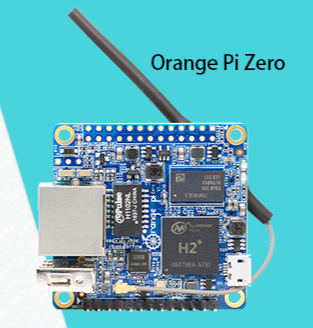
\includegraphics[width=0.6\textwidth]{images/OPIZero.png}
	\caption{Orange Pi Zero\cite{orange}, a Node-RED-hez és az MQTT brókerhez használt eszköz}
\end{figure}

Természetesen a végletek között rengeteg lehetőségünk van igényeink szerint választani kiszolgáló hardvert, például egy Orange Pi Zero, 
Raspberry Pi 4, vagy Seeed Odyssey.
Az Orange Pi Zero-ra esett a választásom alacsony ára mellett nyújtott lehetőségei tárháza miatt.

\section{Okos eszközök}

\subsection{Androidos eszköz}
Mivel az Androidos alkalmazások bizonyos könyvtárai és fejlesztői eszközei az alkalmazott Android verziótól függnek, 
így az alkalmazás fejlesztése során kitűzött minimum Android verziót el kell érnie a használni kívánt eszköznek. 
Ebben az esetben a minimum támogatott Android verzió a Marshmallow, azaz Android 6.0. Ez a legrégebbi Android megjelenés 
amit bevett szokásként támogatnak a modern alkalmazások, ennél korábbi verziót támogatni nehézkes, általában nem éri meg, mivel
a felhasználók kevesebb mint 4\%-a használ olyan eszközt, ami 6.0-nál régebbi Androidot futtat\cite{android-versions}.
Ezen a követelményen felül, és hogy képes legyen az eszköz egy hálózathoz csatlakozni, nincs egyéb megkötés a hardverrel
kapcsolatban, mivel a fejlesztés során figyelembe vettem a kisebb kapacitású eszközöket is, az alkalmazásnak
egészen alacsony erőforrásigénye van.

\subsection{ESP 8266}

\begin{figure}[ht]
	\centering
	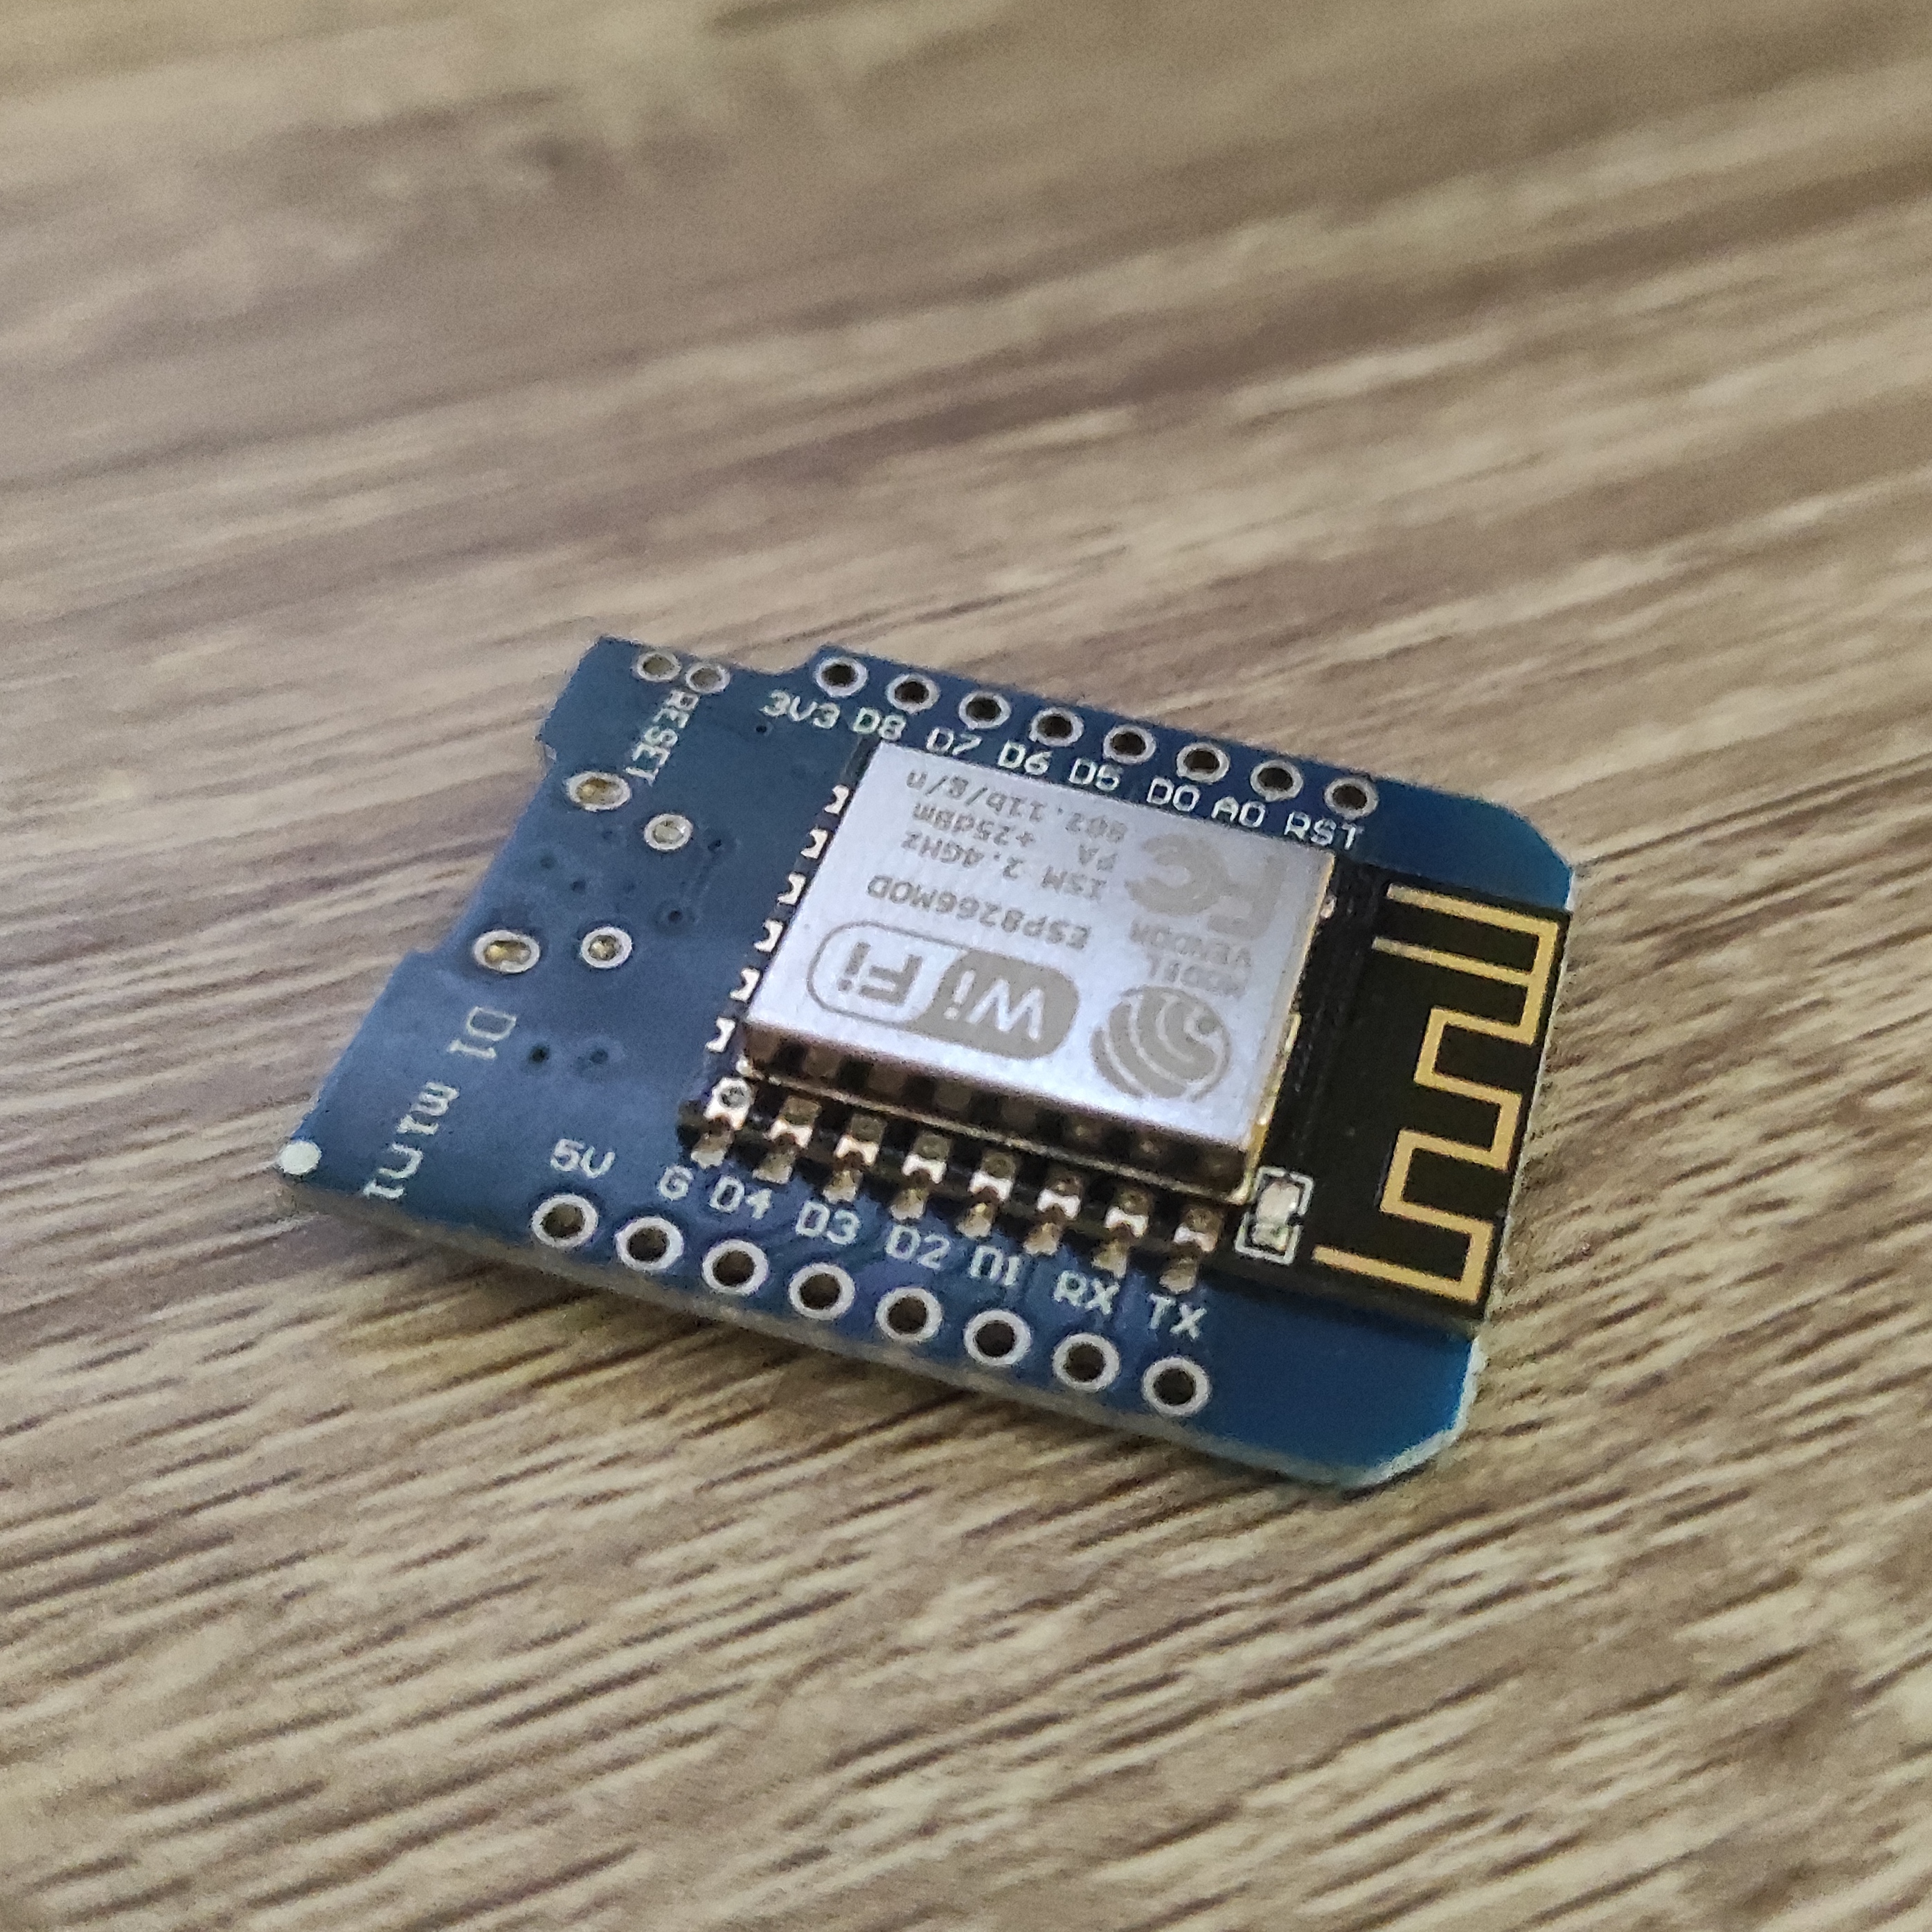
\includegraphics[width=0.6\textwidth]{images/esp.png}
	\caption{ESP 8266}
\end{figure}

Okos eszköz fejlesztésére egy rendkívül olcsó lehetőség az ESP D1 Mini mikrokontroller, ami Arduino nyelven
programozható. WiFi moduljának, hivatalos Arduino MQTT könyvtárnak és rengeteg bővítési lehetőségének
köszönhetően viszonylag egyszerűen okosotthon eszközzé lehet alakítani, vagy akár meglévő eszközöket
is lehet vele okosítani, például egy relé modul irányításával okos kapcsolóként használhatjuk.



\subsection{Egyéb eszközök}
Minden olyan okos eszköz integrálható a rendszerbe, amely képes MQTT protokollon keresztül kommunikálni egy helyi hálózaton.

\chapter{Szoftver}
A teljes rendszer olyan módon van felépítve, hogy a szerver oldali programoktól elvárt, hogy állandó futás mellett lehetőséget 
nyújtsanak bővítésre, konfigurációra és változtatásokra. 
\section{PM2}
Az állandó futást a PM2\cite{pm2} nevű folyamatvezető program biztosítja, akár egy váratlan újraindítás
 vagy áramkimaradást követően az operációs rendszer indulásával elindítja az összes kiszolgálót, amire szükség van,
 megfelelő konfigurációval.

\begin{figure}[ht]
	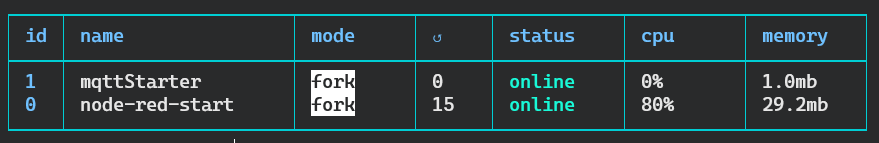
\includegraphics[width=1\textwidth]{images/pm2.png}
	\caption{PM2\cite{pm2} a kiszolgálók automatikus indítására használt eszköz}
\end{figure}

Ez a terminálban futtatható Node.JS eszköz egyszerűen telepíthető NPM vagy Yarn csomagkezelőkkel,
 és azonnal használatba vehető. Lehetőséget nyújt nem csak Node.JS alkalmazások futtatására, 
 de egyéb futtatható fájlok kezelésére is, például shell scriptek futtatására.

\section{Node-RED}
\subsection{Flow}
A Node-RED rendszerben csomópontok elhelyezésével és azok összekötésével lehet egy folyamatábrára hasonlító 
szerkezetet kiépíteni, ami a program viselkedését befolyásolja. Minden csomópont egy funkciót lát el, 
ehhez mérten van a csomópontnak  egy vagy több bemeneti és/vagy kimeneti pontja, 
amin keresztül kommunikál a többi csomóponttal.

Egy ,,flow'' a Node-RED felületén a benne lévő csomópontok és azok kapcsolatát foglalja magában. 
Minden flow reprezentálhat egy házban egy-egy szobát, nagyobb rendszereknél például egy-egy épületet, 
vagy több emeletes épületekben egy-egy emeletet. Ez felhasználható rendszerezési,
kategorizálási vagy szerepköri felosztásra is, teljes mértékben a felhasználótól és a felhasznált
környezettől függ.

\begin{figure}[ht]
	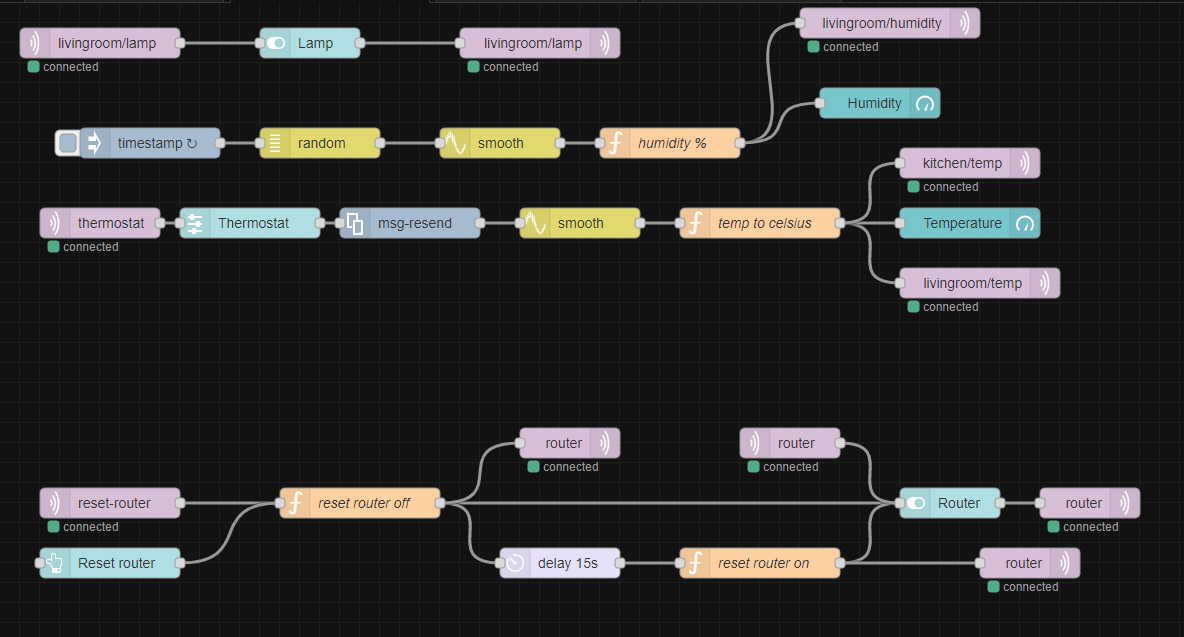
\includegraphics[width=1\textwidth]{images/flow.png}
	\caption{mintaház nappali flow}
	\caption{Egy mintaház kiépítésében a nappaliban található eszközök irányítása}
\end{figure}

Az MQTT csomópontok belső konfigurációja csupán két dolgot vár el felhelyezése során: az MQTT topic, amire az adott csomópont feliratkozik, és az MQTT bróker címe. A bróker címét minden MQTT csomópont megosztja, így a kiszolgáló címének változásakor
elég egy helyen megváltoztatni a címet, az összes csomópont megkapja az új címet és újra tud csatlakozni.

Implementáltam minden szobába egy okos lámpát, hőmérőt és páratartalom mérőt. Ezen felül a nappaliban és a hálószobában vagy egy-egy termosztát, melyeket függetlenül irányíthatunk. Mivel ez a mintaház csak szimuláció, így a szemléltetés érdekében
a hőmérséklet változást egy időintervallum alatt fokozatosan változtatom a termosztát állítást követően, így reprezentálva a való világban a ház fokozatos felfűtését/lehűtését. Szintén szemléltetési céllal a páratartalom mérők
véletlenszerű értékeket vesznek fel, mivel egy bemutató példa házban nem szükséges a valóságnak megfelelő értékeket szimulálni, a rendszer szemléltetése a lényeg.

Az okos lámpa egy egyszerű kapcsolóként jelenik meg a bemutató házban, ez természetesen egy okos kapcsolóval ellátott lámpát reprezentál, melyet irányíthatunk az Androidos alkalmazásból, vagy a webes felületről.

Ezen felül felhelyeztem egy internet router újraindító gombot, ezzel adva példát egy egygombos funkció ellátására, mivel egyszerűbb egy újraindítás gombot megnyomni, 
mint kapcsolóként kezelni és a felhasználóra bízni, hogy ne kapcsolja vissza idő előtt a router-t, így megelőzve az esetleges 
késés által előidézett idő kimaradás eltörlését, mivel az MQTT sorban küldi az üzeneteket, ha a rendszer lelassul egy pillanatra, 
lehet, hogy két üzenet, amit a felhasználó egymástól eltérő időpontban küldött el, mégis egyszerre érkezik a kiszolgálóhoz.

Ezt a webes szerkesztő felületet a helyi hálózaton a kiszolgáló eszköz IP címén, a konfigurációban megadott portszámon (alapbeállítás szerint 1880) lehet elértni.
Az itt végzett változtatások csak akkor kerülnek a futási környezetbe, ha a ,,Deploy'' feliratú gombot megnyomjuk, különben minden változtatás
csak a felületen történik, átmenetileg van mentve, hogy közben a szolgáltatás az előző verzióval tovább tudjon futni, így
állandó elérést és irányítást biztosítva a már felcsatlakozott okos eszközök számára.

Ez a viselkedésforma
rendkívül előnyös mind a fejlesztés mind egy meglévő rendszer bővítése során, mivel az új funkciók
fejlesztése során nem kell a már meglévő funkcionalitást felfüggeszteni.

\subsection{Dashboard}
A Node-RED lehetőséget nyújt egyéb csomópontok telepítésére, melyeket felhasználók vagy egyéb entitások fejlesztettek. 
Egy ilyen csomópont kollekció a Node-RED Dashboard\cite{dashboard}, mely által lehet készíteni egy webes felületet, amin keresztül lehet szemléltetni, irányítani a rendszer elemeit. 
\begin{figure}[ht]
	\centering
	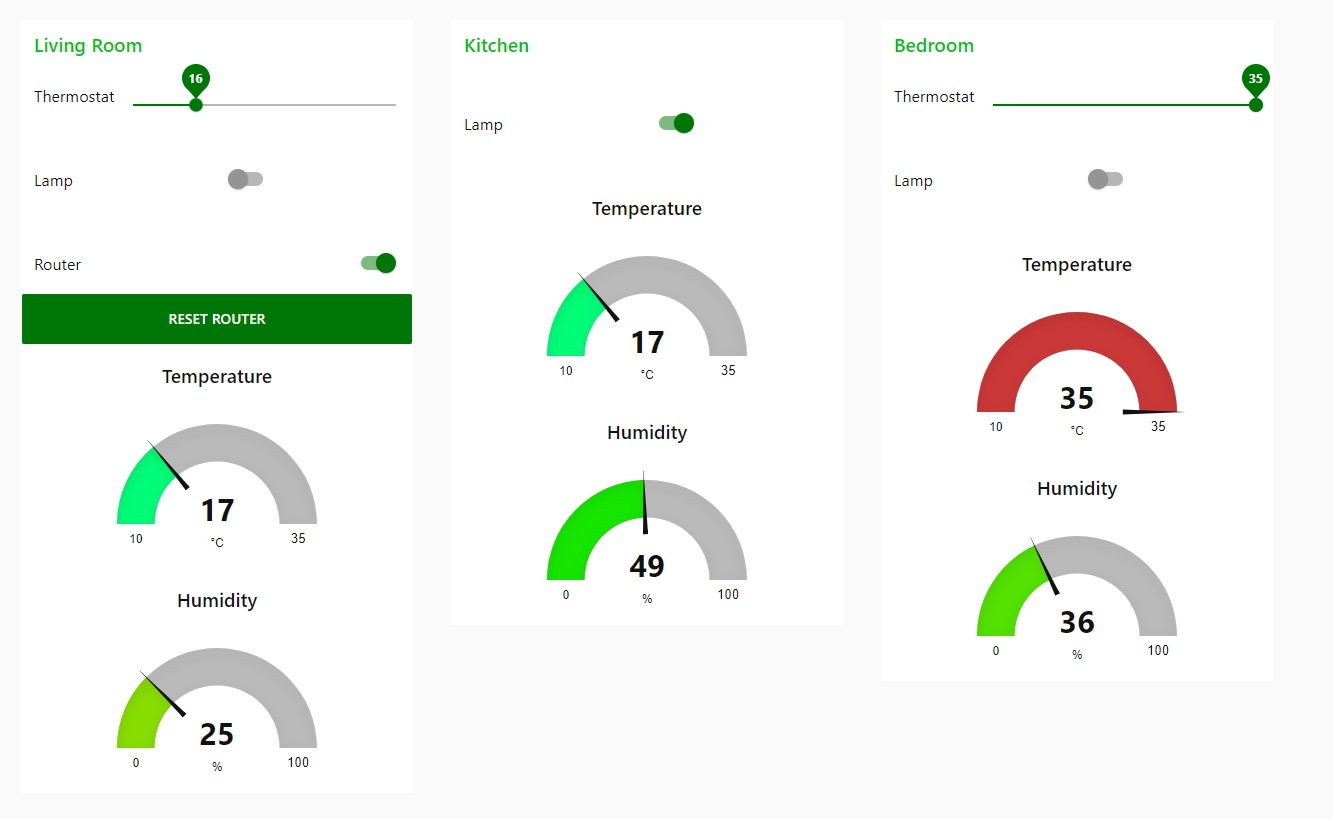
\includegraphics[width=0.8\textwidth]{images/dashboard.jpg}
	\caption{A Node-RED Dashboard, szobákra bontva, példa eszközökkel ellátva}
\end{figure}


Ez nem olyan rugalmas, mint az Android alkalmazás, mivel minden
elemet kézzel kell felvenni a felületre, majd minden konfigurációját és interakcióját a flow szerkesztőben kell kézileg megadni, minden elemet külön fel kell programozni.

\section{MQTT}
\subsection{Bróker}
MQTT brókernek az Eclipse Mosquitto\cite{mosquitto}-t választottam, mivel egy jól ismert alapítvány által fejlesztett, teljesen nyílt forráskódú multi-platform projekt,
melyben különös figyelmet fordítottak az erőforrásokkal való spórolásra, így a gyengébb egykártyás számítógépeken való alkalmazását megkönnyítve. 

Szintén előnyt jelentett választásom során a jó minőségű dokumentáció, mely alapján
viszonylag zökkenőmentes volt a telepítés és a konfiguálás és a hibaelhárítás.
\subsection{Konfigurálás}
Mivel a konfigurációs fájlban meg kell adni a brókernek, hogy mely címen fog csatlakozási kérelmeket és üzeneteket kapni,
készítettem egy olyan shell scriptet, mely minden indításnál egy új, naprakész konfigurációs fájlt készít a bróker indítása előtt.

\lstset{language=bash} 
\label{configGenerator}
\begin{lstlisting}[frame=single]
echo -n "listener 1883 " > mqtt.conf; ip -4 addr show eth0 | grep -oP '(?<=inet\s)\d+(\.\d+){3}' >> mqtt.conf echo $"allow_anonymous true" >> mqtt.conf
\end{lstlisting}

Ez a shell script generál egy olyan konfigurációs fájlt, ami a következőket állítja be:
\begin{itemize}
	\item 1883-as porton várja az üzeneteket
	\item Lekérdezi a kiszolgáló számítógép IPv4 címét, amit egy regex szűrőn keresztül formázom megfelelő módon és a portszám után illesztem be, előírás szerint.
	\item Végül engedélyezi az anonim kapcsolatokat. Mivel ez a rendszer egy helyi hálózatra van tervezve, nem jelent biztonsági kockázatot az autentikáció nélküli kapcsolat, ezt kiváltja az MQTT ID rendszer.
\end{itemize}

\section{Android}
\subsection{Activity}
Az Android ,,aktivitásokra'' bontja a kódot, melyek a hozzájuk tartozó ,,töredékek'' alappilléreként szolgál.
Fő célja az aktivitásokra bontásnak az erőforrások megspórolása, minden aktivitás egy specifikus feladatkört lát el, 
miközben a másik aktivitások a háttérben leállnak, amíg nem lépnek újra használatba. Az én esetemben egy fő aktivitás
látja el az alapvető feladatait az applikációmnak, mivel ennek a fő aktivitásnak a kiszolgálóval való kapcsolattartás és
a felhasználói adatok tárolása, így több aktivitásra bontani ezt csak feleslegesen bonyolítana mind a program logikáján,
mind az átláthatóságán.

Az Android rendszer alapjáraton 4 fő ,,szálat'' különböztet meg:
\subsubsection{Main Thread}
A fő szál. Ez az alkalmazás indításakor az operációs rendszer által nyitott szál, mely felelős az események kezeléséért,
felhasználói felület megrajzolásáért és egyéb elemek létrehozásáért.
	
\subsubsection{Ui Thread}
A felhasználói felületi szál, ami felelős a felhasználóval való kapcsolat fenntartásáért 
és a felületi eseménykezelésért mint például egy gomblenyomás. Fontos, 
hogy a UI szálat sosem szabad megakasztani hosszú folyamatokkal, 
például hálózati csatlakozás indításával, mivel ilyenkor a felület teljes egészében leáll, 
a felhasználó felé nem reszponzív, nem tud semmilyen eseményt kezelni 
amíg a folyamat ami megakasztotta a szálat be nem fejeződik.
	
\subsubsection{Worker Thread}
Az egyéb többszálas folyamatokat kezelő szál. Ez a szál nyújt megoldást a UI szál megakasztásának elkerülésére,
ezt kell használni hosszabb, nem azonnal ellátható események kezelésére. Felmerül használata során viszon az a
probléma, hogy a felhasználói felületet csakis a UI szálról lehet frissíteni, így nem minden esetben csak ezt
optimális használatba venni. 
	
\subsubsection{Binder Thread}
A kötött szolgáltatások távolról meghívható metódusokat tartalmaznak. Ha a végrehajtott metódusra történő felhívás ugyanabban a folyamatban van, amelyben a kötött szolgáltatás fut, a metódus a hívószalagban hajtódik végre. Ha azonban a hívás egy másik folyamatból származik, akkor a metódus egy olyan szálban kerül végrehajtásra, amelyet a rendszer ugyanabban a folyamatban tart, mint az meghívó.

\subsection{Fragmentek}
A fragment azon része az alkalmazás felhasználói felületének, ami saját felosztását definiálja és kezeli. Saját életciklussal
rendelkezik, viszont egyedülálló elemként nem használható, mindig kell lennie egy tulajdonosának, ami lehet egy másik
fragment vagy activity. Ehhez a tulajdonoshoz kötve jelenhet meg egy fragment felülete hozzá csatolva vagy részévé válva.

A fragmentek célja hogy egy activityn belül különválasztott felhasználói felületet prezentálhassunk, egymástól független
elemekre bontva, így megkönnyítve a felhasználói felület felépítésének procedúráját és az erőforrások megtakarítását.

A fragmentek ideális használati köre egy activityn belüli navigációs elemek által elérni kívánt felületek prezentációja. Mivel egy fragment életciklusa akkor ér véget, amikor a felhasználó egy másik fragmentre váltással felülírja azt, hosszútávú
adattárolásra nem alkalmas, bár erre is vannak beépített megoldások, például a fragmentet tartalmazó activiy szintjén tárolni
az adatokat, vagy a fragmentek belső ,,instance bundle'' változójával kezelni, bár az utóbbi típusmegközései miatt igencsak
korlátozó módszer, de több módszer kombinálása sem kizárt, így mindent olyan módon lehet kezelni, ahogyan az adott esetben optimális.
\subsection{Felhasználói felület}
Az alkalmazásom felhasználói felülete 3 fő fragmentből áll: Home, Settings és Help. A Home fragment a fő interakciós felülete
az alkalmazásnak, itt tölti a felhasználó az ideje nagy részét, itt éri el és irányíthatja a hálózaton található okos eszközöket.

A Settings fragment a kiszolgáló címének megadására, felhasználói profil kiválasztására és a kapcsolat létesítésére
szolgál.

A Help fragment felhasználási segítséget nyújt a felhasználó számára, ha nem biztos az alkalmazás működésének rendjében,
ezen leírás alapján tud tájékozódni a rendeltetésszerű felhasználásról.

Az alkalmazásban található minden felhasznált grafikai elem a Material Design\cite{material} előírásait követve készültek,
ami a Google által kifejlesztett design nyelv. Eredetileg a Google által használt kártya alapú design továbbfejlesztése
reszponzív animációk, átmenetek és mélységi effektek (megvilágítás, árnyékok) implemetálásával. Ezeket az előírásokat és
kész elemeket felhasználva biztosítottam, hogy a felhasználói felület rögtön ismerős hatást keltsen, könnyen lehessen rajta
eligazodni és hogy a jövőben kevésbé tűnjön elavultnak, régimódinak.


\subsubsection{Home}
A Home fragment szolgál az eszközök kezelésére, irányítására, adatok prezentálására.
A felület jobb alsó sarkában található ,,Floating Action Button'', vagy FAB megnyomására a felhasználó feliratkozhat egy MQTT
topicra, majd kiválaszthatja a létrehozandó kártya interakciós típusát. 

Ha sikeresen feliratkozik egy topicra, a felületen létrejön
egy ,,kártya'' a kiválasztott interakciós típussal, például egy csúszkával, gombbal vagy kapcsolóval. Ezt követően a felhasználó a
kártyán keresztül tudja kezelni az adott topicot használó okos eszközöket. 

Ha a felhasználó el szeretné távolítani a kártyát a felületről,
egy hosszú érintéssel a kártya bármely részére előidéz egy ,,Unsubscribe'' kontextusi gombot, mellyel törölheti a kártyát a felületről.

\begin{figure}[ht]
	\centering
	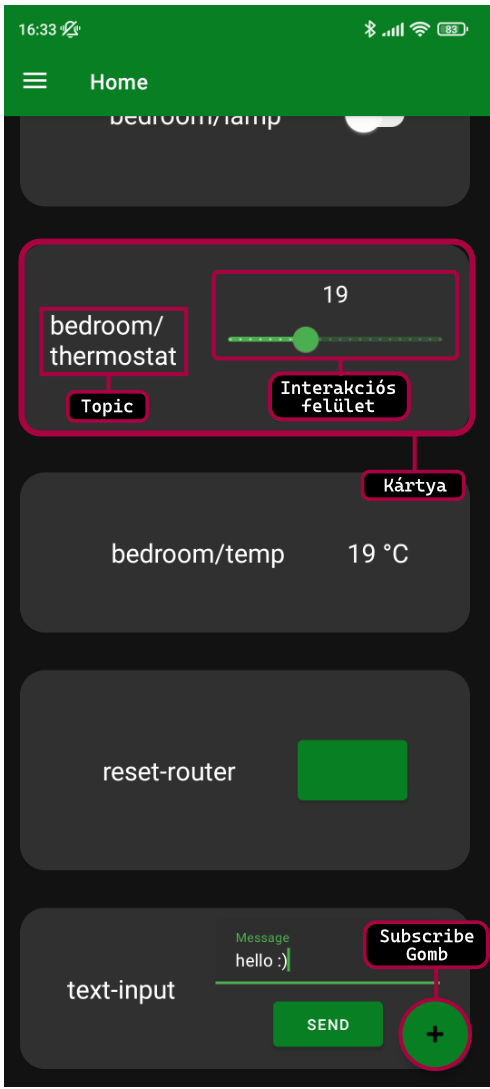
\includegraphics[width=0.5\linewidth]{images/home_anatomy.png}
	\caption{A Home fragment elrendezése és elemei}
	\label{fig_home_anatomy}
\end{figure}
	
\subsubsection{Settings}
A Settings fragment a kiszolgálóhoz való csatlakozásra és a felhasználói profil beállítására szolgál.

A felületen található két beviteli mező. Az elsőbe a felhasználói profil elnevezését, a másodikba a kiszolgáló címét
kell megadni, majd a ,,Connect'' gomb megnyomására az alkalmazás  kapcsolatot létesít a kiszolgálóval és ellenőrzi, hogy
létezik-e már a megadott néven felhasználói profil. Ha már létezik, az alkalmazáson belüli tárba betölti az elmentett adatokat,
viszont ha nincs, létrehozza azt.

A ,,Delete Profile'' gomb egy új ablakban, legördülő menüből kiválasztható profilok listájából törli azt, amelyet a
felhasználó kiválaszt.
\begin{figure}[ht]
	\centering
	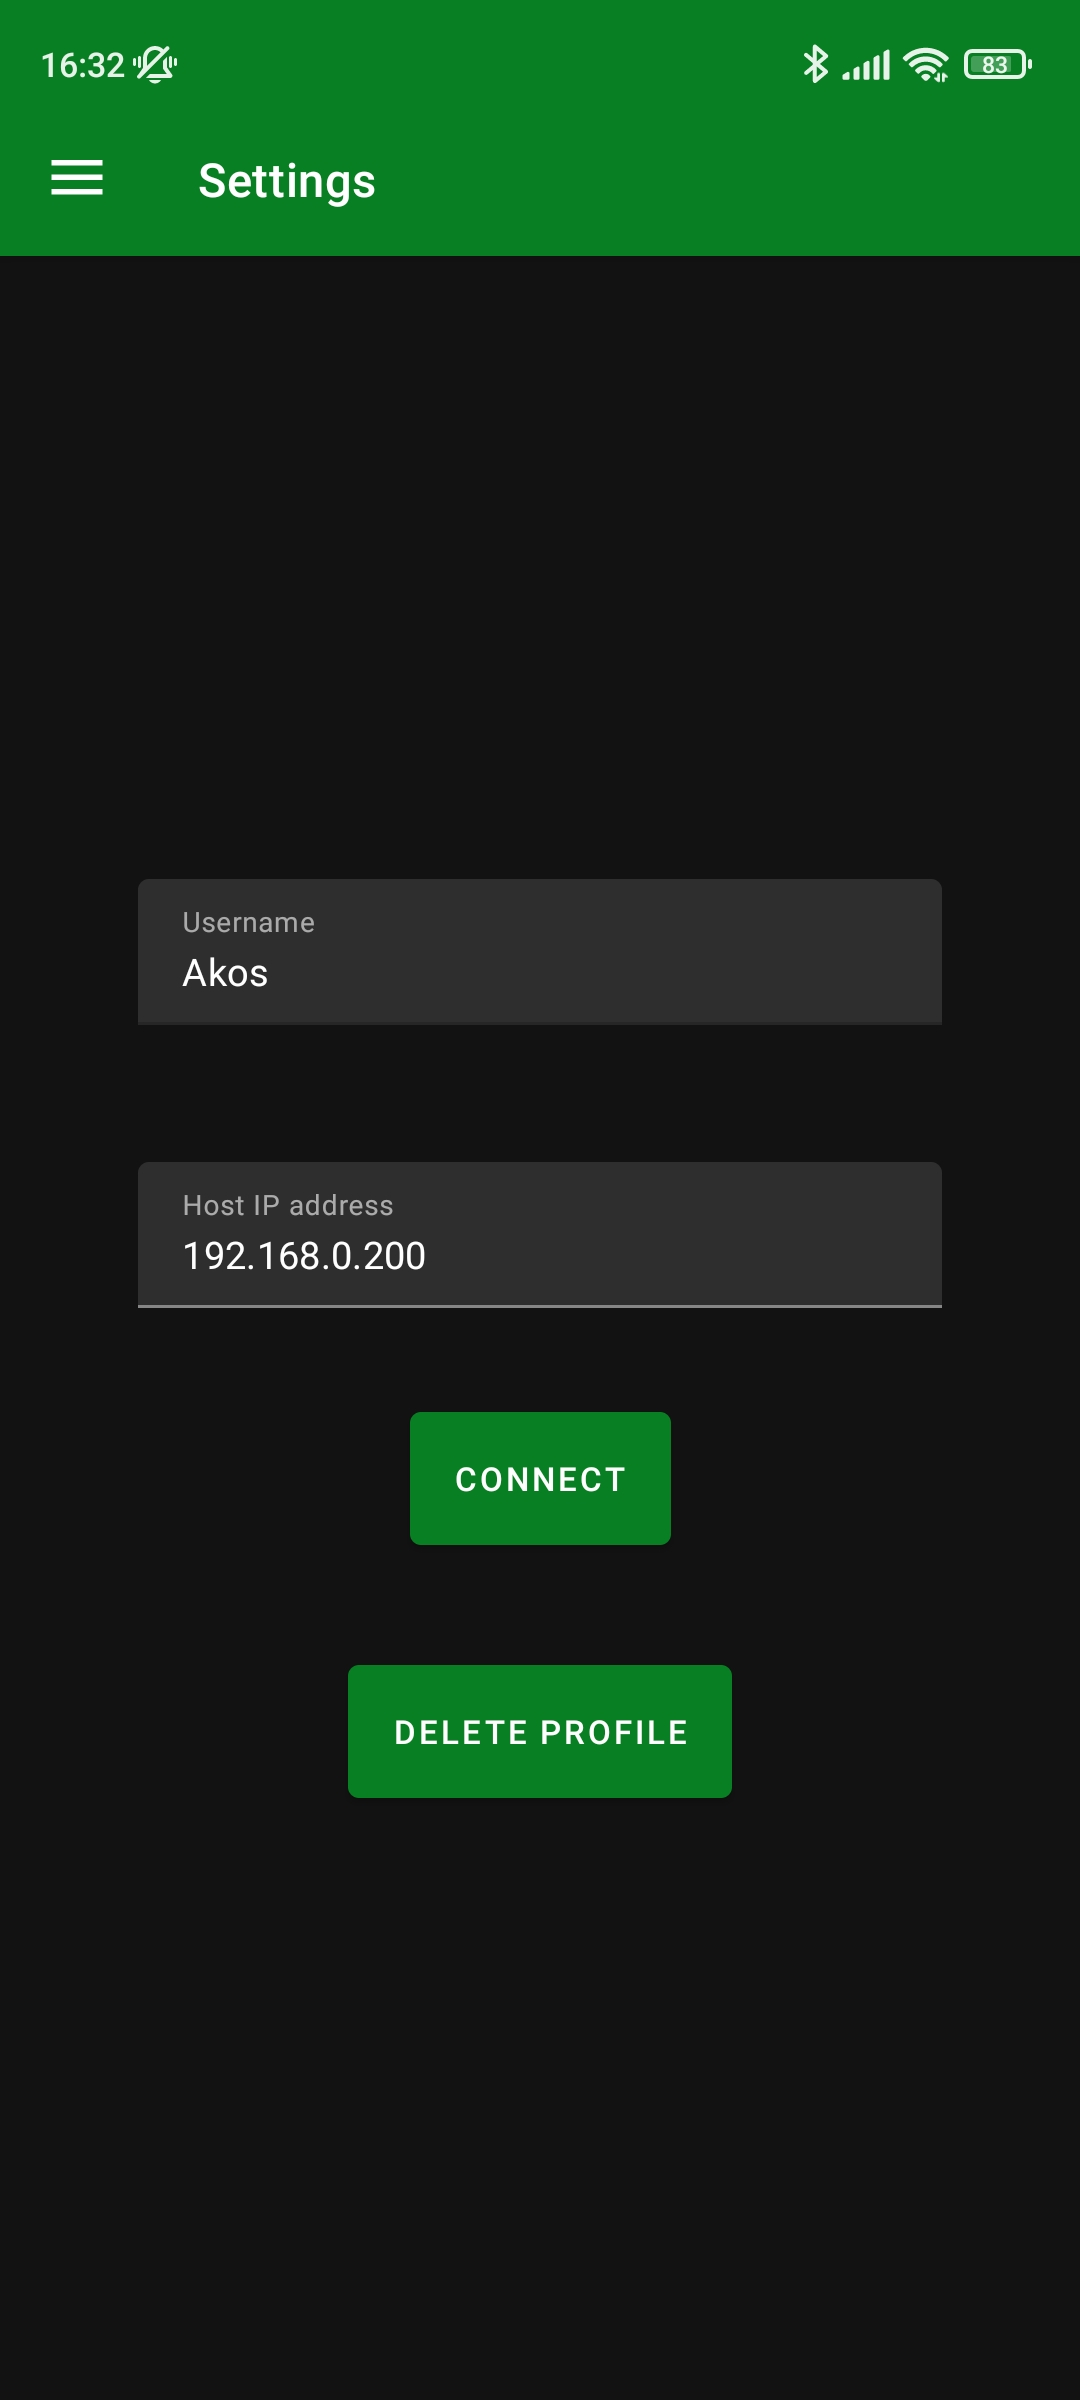
\includegraphics[width=0.5\linewidth]{images/connect.jpg}
	\caption{A beállításokat tartalmazó fragment}
\end{figure}

Az itt megadott értékeket az alkalmazás eltárolja, így a következő indításkor ezek a mezők már az előző használatkor
alkalmazott értékekkel kitöltve jelennek meg, így megkönnyítve és felgyorsítva az alkalmazás használatát.

\subsubsection{Help}
A help fragment tartalmazza a felhasználói útmutatót. Itt lehet tájékozódni az alkalmazás rendeltetésszerű használatáról,
a funkciók céljáról, használatáról és az esetleges problémák megelőzéséről, kijavításáról.

A help fragment szintén kártyákra osztja a felületet a könnyű és gyors átláthatóság érdekében és a
konzisztencia fenntartásáért.

\subsection{Kapcsolat}
Az MQTT kapcsolatot Android oldalon szintén az Eclipse Foundation megoldását használom, a paho\cite{paho} nevű,
nyílt forráskódú MQTT kliens Android implementációját, a Garadle rendszeren keresztül összeállított,
Maven repositoryból letöltött forrás csomagját importálva.

A kapcsolat 60 másodperces időtúllépést elérve felbontódik, ha nem kap választ a kiszolgáló az életben tartó
jelre. Ezért a kapcsolat létrehozása pillanatában a kliens entitását eltárolom egy activity szintű változóban,
így a kapcsolat addig él, amíg a felhasználó használja az alkalmazást, vagy nem zárja be több mint 1 percre.

\lstset{language=Java}  
\begin{lstlisting}[frame=single]
MqttAndroidClient client = new MqttAndroidClient(this.getApplicationContext(),
"tcp://" + mqttAddress + ":1883", clientId);

client.connect(null, new IMqttActionListener() {
	@Override
	public void onSuccess(IMqttToken asyncActionToken) {
		mqttClient[0] = client;
	}

	@Override
	public void onFailure(IMqttToken asyncActionToken, Throwable exception) {
		Toast toast = Toast.makeText(getApplicationContext(),
				"Failed to connect to " + mqttAddress, Toast.LENGTH_SHORT);
		toast.show();
	}
});
\end{lstlisting}

Ez a kapcsolat aszinkron módon jön létre, így nem kell megállítani a felhasználót, amíg nem jön létre a
kapcsolat, vagy hibát eredményez a csatlakozás, például hibás címet adott meg a felhasználó vagy
a kiszolgáló nem fut. Erről természetesen a felhasználó egy üzenetet kap egy ,,toast'' formájában, ami egy
kis méretű felugró üzenet, ami kiváló lehetőséget nyújt a felhasználóval való kommunikációra.

\subsection{Kártyák}
A jelenlegi verzióban 6 típusú kártya használatára van lehetőség, de ez a jövőben egyszerűen bővíthető:
\begin{itemize}
	\item Text: Szimpla szöveges feliratot prezentál, felhasználható például hőmérő értékének kijelzésére.
	\item Button: Egy gombot tartalmaz, ami az adott topic-ra egy "1"-es üzenetet küld, amit a kiszolgáló
	dolgoz fel.
	\item Checkbox: Egy jelölőnégyzet, mely "on" és "off" üzenetet küld a kiszolgálónak állapota szerint.
	Lehet használni állapotjelzőnek vagy kapcsolónak.
	\item Switch: Egy kapcsoló, mely szintén "on" és "off" üzenetet küld a kiszolgálónak állapota szerint,
	így logikusan alkalmazható például okos lámpa kapcsolójaként.
	\item Input: Egy beviteli mezőt tartalmaz, amibe tetszőleges szöveget vagy számot írhat a felhasználó,
	majd az alatta lévő gomb érintésével elküldi a tartalmát az adott topic-ra. Használható például LED-es
	tábla feliratának módosítására.
	\item Slider: Egy csúszka, amelynek minimum és maximum értékeit a felhasználó határozza meg, az ez
	által nyújtott sokoldalúságából eredendően lehet használni például termosztát beállítására, vagy
	okos lámpa fényerejének módosítására.
\end{itemize}

Egy kártya felépítése a korábban látott ábra szerint (\ref{fig_home_anatomy}) két félre bontódik.
Bal oldalán található a topic felirata, amelyre az adott kártya feliratkozott. 

A jobb oldalán található
a felhasználó által választott interakciós felület, melyen keresztül tud kommunikálni az alkalmazás a
kiszolgálóval az adott topic-on. 

Minden kártya egymástól teljesen független, így például több kártya ugyan
arra a topicra képes feliratkozni, nem okoz problémát, minden kártya feldolgozza a rá vonatkozó,
azaz a topicra érkező üzeneteket.

Egy törölni kívánt kártyát a hosszú érintésével előidézhető ,,Unsubscribe'' gomb megnyomásával tudunk
eltávolítani a felületről. Ez nem csak vizuálisan szünteti meg az adott kártyát, de a topicról is
leiratkozik, amit eddig használt, így azt a minimális erőforrást is felszabadítva amit elfoglalt. 

Mielőtt egy kártya sikeres feliratkozás eredményeként létrejön, több adatfeldolgozási lépést kell megtenni. 
Vegyünk példának egy kapcsoló típusú kártyát:


\lstset{language=Java}  
\begin{lstlisting}[frame=single]
private void createCard(LinearLayout layout, List<String> savedCardData, int type) {
    ViewGroup mqttCard = (ViewGroup) this.getLayoutInflater().inflate(type, null);
    TextView topicDisplay = (TextView) mqttCard.findViewById(R.id.text_topicDisplay);
    registerForContextMenu(mqttCard);
    topicDisplay.setText(savedCardData.get(0));
\end{lstlisting}

A kártya létrehozó metódusa megkapja paraméterként a Home fragment alap elrendezését, amiben majd el kell
helyeznie az új kártyát, egy listát, ami tartalmazza a profilban tárolt kártyák adatát, így ha már
volt a profilban mentett adat, azt visszaállítja a program, nem kell újból azokat megadni, és végül
megkapja a kártya típusát, mely alapján kiválasztja a program, hogy milyen interakciós felületű kártyát
hozzon létre.

Ezt követően inicializálja a kártya struktúra alapját, a topic kijelző szövegét, és elkezdi a kártyatípus ellenőrzését.

\lstset{language=Java}  
\begin{lstlisting}[frame=single]
switch (type) {
	case R.layout.mqtt_card_switch:
		SwitchMaterial switch_data = (SwitchMaterial) mqttCard.findViewById(R.id.switch_data);

		if (!savedCardData.get(2).equals("null")) {
			switch_data.setChecked(savedCardData.get(2).equals("on"));
		}
		switch_data.setOnClickListener(view -> {
			String message = switch_data.isChecked() ? "on" : "off";
			publishMessage(((MainActivity) getActivity()).getClient(), savedCardData.get(0), message);
		});
		layout.addView(mqttCard);
		break;
\end{lstlisting}

Miután a kártyatípus eldöntésre került, inicializálja a kártya létrehozásához szükséges változókat, majd ellenőrzi, hogy volt-e már az adott topicon ilyen típusú kártya mentve.
Ha a létrehozandó kártya nem egy mentett állapotból kerül visszahelyezésre, akkor egy alapbeállítás 
szerinti kezdőértéket vesz vel, ellenkező esetben, ha volt mentett adat az adott kártyáról, azt állítja be kezdőértéknek
(ebben az esetben hogy milyen állapotban volt utoljára a kapcsoló).

Ezt követően létrejön az interakciós felület ,,figyelője'', mely megadja, hogy az adott felület használata
milyen módon reagáljon, ebben az esetben a kapcsoló állapotváltozása küld egy ,,on'' vagy ,,off'' üzenetet a
kiszolgáló számára, állásától függően.

Végül a kártya felkerül a felhasználói felületre a beállított paraméterek szerint.

\subsection{Kommunikáció}
A kártyák és a kiszolgáló közötti kommunikációt egy ,,publishMessage'' nevű metóduson keresztül továbbítom
az alkalmazásból a bróker felé. Ennek a metódusnak szüksége van egy kliens példányra, melyet az activity tárol
csatlakozást követően, a topicra, amire az üzenetet kívánjuk közzétenni és végül természetesen maga az üzenet, amit
el kívánunk küldeni.

Az üzenetek tartalmát minden kártyatípus interakciós pontjának saját kódja határozza meg, például
a kapcsoló típusú kártyának ,,on'' és ,,off'' állapotával megegyező szöveges üzenetet küld, a csúszka típusú
a beállított számértékét, a beviteli mezős kártya pedig természetesen a felhasználó által megadott üzenetet.

\lstset{language=Java}
\begin{lstlisting}[frame=single]
switch_data.setOnClickListener(view -> {
                    String message = switch_data.isChecked() ? "on" : "off";
                    publishMessage(((MainActivity) getActivity()).getClient(), savedCardData.get(0), message);
                });,
\end{lstlisting}

Az üzenetek fogadását egy ,,messageRecievedHandler'' nevű metódus kezeli, amit az MQTT kliens callback metódusa
hív meg a ,,messageArrived'' belső metódusából, azaz minden beérkezett üzenet hatására, átadva a beérkező üzenet topicját és tartalmát.

A beérkező üzenet topicját először ellenőrzi, hogy egyezik-e az aktuálisan vizsgált kártya topicjával, majd
összehasonlítja a kártya típusát az elvárt típussal. Ha minden egyezik, akkor a dekódolt üzenet tartalmát
kártyatípusnak megfelelően jeleníti meg, vagy állítja be a kártyán található interakciós elem állapotát.

\lstset{language=Java}
\begin{lstlisting}[frame=single]
if (topicDisplay.equals(topic)) {
	if (activeElement instanceof SwitchMaterial) {
		SwitchMaterial switchView = cardList.getChildAt(i).findViewById(R.id.switch_data);
		switchView.setChecked(decodeMQTT(message).equals("on"));
	}
}
\end{lstlisting}

Az MQTT üzenetek dekódolása egy egyszerű String-é alakítás, mivel a beérkezett üzenet egy saját típusú, MttMessage
objektum amiben egyéb adatok mellett az üzenet egy byte tömbben tárolódik, amit kevésbé egyszerű és gyors minden
feldolgozásnál kezelni, ezért egy új szöveges változót építek a tartalmából.

\lstset{language=Java}
\begin{lstlisting}[frame=single]
private String decodeMQTT(MqttMessage msg) {
	return new String(msg.getPayload(), StandardCharsets.UTF_8);
}

\end{lstlisting}

A kapcsolat a kiszolgálóval addig él, amíg az alkalmazás tud válaszolni a kiszolgáló által közvetített jelre,
ami azonosítja, hogy mely eszközök vannak aktív állapotban. Ha erre az üzenetre az alkalmazás nem tud válaszolni,
azaz a felhasználó bezárta azt, 60 másodpercen belül lezáródik a kapcsolat. Ezt a kapcsolatbontást az alkalmazás
közli a felhasználóval, majd felajánlja az újracsatlakozás lehetőségét. Ha a felhasználó nem él a lehetőséggel,
a kapcsolatot újból a Settings fragmentről kell létesíteni, vagy egy kártyán keresztül
új üzenetet kell küldenie a kiszolgáló felé, ami a küldést megelőzően megpróbálja visszaállítani a kapcsolatot.

\subsection{Adattárolás, Profilok}
A kártyaadatok profilonkénti tárolása egy szöveges fájlba való kiírással oldottam meg, olyan formátumban, hogy a fájl
neve a felhasználói profil megadott neve, a tartalma pedig minden kártya amit a felhasználó létrehozott, a következő
formában felbontva: Topic:Kártytípus:Tárolt adat.

Minden kiírás esetén ellenőrzöm, hogy már szerepel-e a fájlban a jelenleg mentésre kijelölt kártya, így elkerülve
felesleges kiíratási folyamatokat, ha már létezik, mivel ebben az esetben felesleges lenne kitörölni és újra kiírni.

Ez az ellenőrzés viszont csak a kártya topicra és típusra vonatkozik, mivel a tárolt adat folyamatosan változik.
Az ellenőrzés során megkeresem az összes olyan elmentett kártyát, ami ugyanazt a topicot és kártyatípust tartalmazza,
majd csak azt a sort írom felül a friss adatokkal, így nem kell a teljes fájlt újraírni csak egy sor módosításáért.

Friss profiloknál, mivel egy üres fájl jön létre, a kereső algoritmus hibát dobna, mivel nem tud üres sorokban
keresni, ezért erre az esetre egy külön elágazást implementáltam, ami szimplán kiírja a menteni kívánt kártya adatait,
mivel ebben az esetben biztosak lehetünk abban, hogy még nem tartalmazza a fájl ezt a kártyát, ezért átugorhatjuk az
ellenőrzést.


\lstset{language=Java}  
\begin{lstlisting}[frame=single]
public void addCardDataToPersistentStorage(String topic, String cardType, String cardData) {
	boolean found = false;
	int i = 0;
	if (cardDataStore.size() == 0) {
		this.cardDataStore.add(topic + ":" + cardType + ":" + cardData);
	}
	do {
		String[] part = this.cardDataStore.get(i).split(":", 0);
		if ((part[0] + ":" + part[1]).equals(topic + ":" + cardType)) {
			this.cardDataStore.set(i, topic + ":" + cardType + ":" + cardData);
			found = true;
		}
		i++;
	}
	while (!found && i < cardDataStore.size());

	if (!found) {
		this.cardDataStore.add(topic + ":" + cardType + ":" + cardData);
	}

	writeToFile(this.username + ".txt", this.cardDataStore);
}
\end{lstlisting}

A kártyák adatain kívül az alkalmazás tárolja az utoljára használt felhasználónevet és a kiszolgáló címét.
Ezt az Android sajátos ,,SharedPrefrence'' API eszközeivel tárolom, ami kulcs-érték párokat tárol, melyeket csak az
alkalmazáson belül lehet elérni.
Mivel ez a rendszer kis mennyiségű adatok tárolására célzott eszköz, így a kártyák adatainak tárolására nem lenne
alkalmas, viszont a felhasználónév és kiszolgáló címének tárolását beolvasztani a kártyaadat tárolására szolgáló
fájlba rendezetlen és bonyolultnak tűnt, ezért választottam szét a két tárolási módot.

A profilok törlésére a Settings fragmenten található ,,Delete Profile'' gomb megnyomásával van lehetőség,
ami kilistázza az összes profil fájl címét egy legördülő menüben, majd a felhasználó egy profil kiválasztása után
törölheti azt a ,,Delete'' gomb segítségével.

Egy létező profilnév megadása a csatlakozás során azt eredményezi, hogy a profil fájlból a program beolvassa a felhasználó nevén
tárolt kártyaadatokat, amit elhelyez egy memóriában tárolt listában, majd azt továbbítja a Home fragment számára, ami
adatrészekre tördelve feldolgozza azt és létrehozza az összes kártyát, amit a felhasználó az utolsó használata során
elmentett.

A memóriában tárolt kártyaadatok listájának minden eleme egy teljes kártyát tartalmaz, aminek feldolgozásához részelemekre
kell tördelni, majd ezeket a részelemeket felhasználva építem fel a kártyákat. Vegyük példának a csúszka típusú kártyát:

\lstset{language=Java}
\begin{lstlisting}[frame=single]
List<String> sliderSubData = Arrays.asList(savedCardData.get(2).split("\\."));
TextView sliderDataDisplay = mqttCard.findViewById(R.id.slider_data_display);

String rangeMin = sliderSubData.get(0);
String rangeMax = sliderSubData.get(1);
String currentVal = sliderSubData.get(2);

slider_data.setValueTo(Float.parseFloat(rangeMax));
slider_data.setValue(Float.parseFloat(currentVal));
slider_data.setValueFrom(Float.parseFloat(rangeMin));

sliderDataDisplay.setText(currentVal);
layout.addView(mqttCard);
\end{lstlisting}

A kártyák létrehozásakor a metódus megkapja az adott kártyára vonatkozó adatokat egy ,,savedCardData'' listában, aamelynek
3 eleme van: topic, kártya típus és a kártyáról tárolt adat. A csúszka esetében a kártyáról tárolt adatot tovább kell tördelni,
mivel nem csak az utolsó állapotát kell tárolni, hanem a felhasználó által megadott minimum és maximum felvehető értékeit is.
Ezeket az extra kártyaadatokat kinyerve beállítom a csúszka minden tulajdonságát, majd létrehozom a kártyát.

\section{ESP Okos eszköz}
Egy ESP D1 Minit használtam egy hálózaton lévő okos eszköz szemléltetésére, amit olyan módon programoztam fel, hogy egy
okos lámpa funkcióit lássa el. Az Adafruit MQTT Könyvtárát\cite{adafruit} kihasználva egészen egyszerű módon lehet csatlakozni
egy helyi hálózaton található MQTT brókerhez, majd feliratkozni egy vagy több topicra, melyen természetesen kétirányú
kommunikációra van lehetőségünk. 

Ebben az esetben az eszköz egyszerűen vizsgálja az általa feliratkozott topicon érkező
üzeneteket, majd a szemléltetés érdekében az eszköz beépített LED-jének állapotát az üzenetnek megfelelően változtatom.
Ezt természetesen valós eszközöknél minimális változtatásokkal okos kapcsolóként lehet alkalmazni, vagy a kód kibővítésével
egyéb, bonyolultabb funkciók ellátására is teljesen alkalmas.

\lstset{language=C++}
\begin{lstlisting}[frame=single]
void loop() 
{
	Adafruit_MQTT_Subscribe *subscription; 
	while(subscription = mqtt.readSubscription(10)){
		String message((char *)bedroom_lamp.lastread);
		if(message == "on"){
			Serial.println("got on msg");
			digitalWrite(ledPin, LOW);
		}
		if(message == "off"){
			Serial.println("got off msg");
			digitalWrite(ledPin, HIGH);
		}     
		delay(10);
	}
}
\end{lstlisting}

\section{Tesztelés}

\subsection{Reszponzivitás}
A fejlesztés során az alkalmazást több típusú tesztelésnek tettem ki. A felület reszponzivitása már az első pillanattól
fontos pontja volt a fejlesztésnek, így különös figyelmet fordítottam mindenféle eszköz típuson való tesztelésre, ellenőrizve
az elemek helyes méretezését, viselkedését, elhelyezkedését, elérhetőségét. Ebben nagy segítséget nyújtottak az 
Android Studio fejlesztői környezet beépített design eszközei és a tetszőleges formátumú eszközök emulálása. 

A reszponzivitás implementálásában sokat segített a már korábban említett Material Design\cite{material} előírások betartása,
de így is felbukkantak problémák a fejlesztés során, mint például a képernyő elforgatása során a felület 
nem hívta meg a rendszer szintű felület elrendezés frissítéséért felelős metódust, 
így minden felhasználó által létrehozott kártya törlésre került. Ez egy jól ismert probléma az Android rendszerben, 
így egyszerűen találtam megoldást, egy a Fragment osztály által örökölt metódus felülírásával.

\lstset{language=Java}  
\begin{lstlisting}[frame=single]
@Override
public void onConfigurationChanged(Configuration newConfig) {
	super.onConfigurationChanged(newConfig);
}
\end{lstlisting}
\subsection{Hibakezelés}
Mivel a rendszer erősen támaszkodik hálózati kapcsolatra, így sok hibakezelést kellett implementálni az esetleges
lecsatlakozások, rosszul címzett üzenetek, újracsatlakozások és egyéb hálózati műveletek pontjaira. Ezeken a pontokon
exception kezeléssel és naplózással íratom ki a hibát, és ahol szükségesnek éreztem, a felhasználó felé is továbbítottam
a hibaüzenetet, természetesen olvashatóra formázva, mivel egy átlagos felhasználónak egy exception hibaüzenete
nem biztos hogy érthető. 

A felhasználóval való kommunikációt ilyen esetekben úgynevezett ,,Snackbar''-al, vagy ,,Toast''-al
valósítottam meg, melyek a képernyő alján megjelenő rövid üzenetekben közlik a keletkezett hiba forrását, legyen az
kapcsolati vagy akár felhasználói hiba, például egy üresen hagyott beviteli mező.

\subsection{Erőforrás felhasználás}
A fejlesztés során az erőforrások felhasználása is figyelembe lett véve, mivel az MQTT egyik legnagyobb előnye
az alacsony erőforrás igénye. Az alkalmazás  futása közben valós idejű méréseket analizálva több olyan
erőforrás igényes folyamatot is felismertem, melyek újraírása és optimalizálása után észrevehetően növekedett
az applikáció reszponzivitása.

Az alkalmazás legfrissebb verziója stressz-teszt alatti maximum memóriaigénye 130MB, ami alacsonynak számít, azt
figyelembe véve, hogy a mai okostelefonok memória kapacitása 8GB alá ritkán esik.
\begin{figure}[ht]
	\centering
	\label{profiler}
	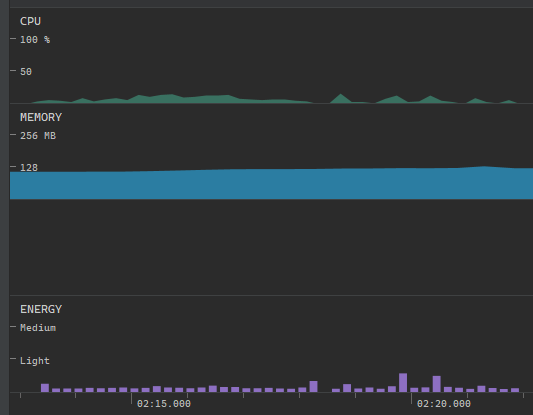
\includegraphics{images/profiler.png}
	\caption{Az app futása közben felhasznált erőforrások}
\end{figure}

A \ref{usage}-as ábrán látható, hogy az alkalmazás memóriaigényének majdnem egyharmadát a grafikai csomagok teszik ki.
A processzorhasználat tesztjeim során maximum 12\%-ot ért el, de tipikus használat alatt 6-7\% volt ez az érték.

Az MQTT magához hűen rendkívül alacsony mennyiségű processzorhasználatot igényelt, nem volt szükség a kommunikáció
optimalizálására.
\begin{figure}
	\centering
	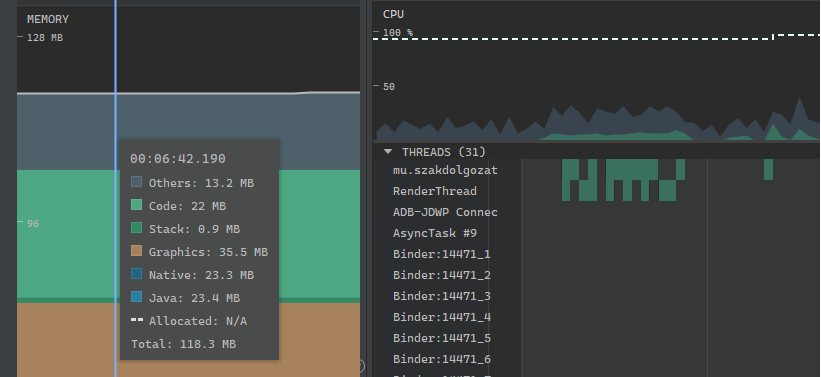
\includegraphics[width=0.9\textwidth]{images/profiler_ram_cpu.png}
	\caption{Az app által felhasznált RAM és CPU, részegységekre bontva}
	\label{usage}
\end{figure}

\chapter{A rendszer működése}
\section{Első indítás}
A Node-RED, a Mosquitto bróker és az Android alkalmazás  is bizonyos fájlokra támaszkodik, melyek az első indításnál
valószínűleg nincsenek jelen. Ez az Android alkalmazás felől nem jelent problémát, hiszen csak annyit jelent, hogy még nincsenek
elmentett felhasználói profilok. A kiszolgáló részéről már kicsit körülményesebb az első indításra való felkészülés,
de ez is inkább időigényes mint bonyolult.
\subsection{Szerver}
A kiszolgáló hardveren természetesen telepíteni kell a Node-RED szolgáltatást az általunk preferált Node.js
csomagkezelővel, például npm, yarn, vagy használhatjuk a Node-RED fejlesztői által biztosított bash scriptet is Linux rendszeren.
A szolgáltatás elindítását követően be kell importálnunk, vagy kézileg felépítenünk a az összes okos eszközre vonatkozó
logikát, kezelést és irányítást. Ezek a flow-k exportálhatóak és importálhatóak egy JSON fájlból, így könnyen hordozható
és megosztható előre megépített flow-k vagy akár teljes házak felépítése.

Az Eclipse Mosquitto MQTT bróker telepítése operációs rendszertől függetlenül egyszerű telepíteni, a Mosquitto
honlapjának letöltési oldalán található instrukciók alapján. A telepítést követően a \ref{configGenerator}-es
beszúrt scriptben látható módon lehet egyszerűen generálni egy konfigurációs fájlt aminek az alkalmazásával
zökkenőmentes a hardver hordozhatóvá tétele, mivel biztosítja a legfrissebb helyi cím átadását a brókernek.

A PM2 rendszer ezeket a lépéseket követően az összes indításkor vagy újraindításkor garantálja a kiszolgálók
indítását, ezért tekinthető egy egyszeri konfigurációs lépésnek.


\subsection{Android}
Az alkalmazás telepítése egyenlőre a proket GitHub oldalán\cite{github}
található ,,Releases'' menüpontban elérhető verziókban letölthető .apk telepítő fájl által lehetséges, de a jövőben
a Google Play Store-on is elérhetővé válik.

Az első indítás nem különbözik más indításoktól, csak a felhasználói profilok hiányában jelentkezhet, de ezek
természetesen a felhasználó igénye szerint generálódnak vagy akár törlődnek, így nem különböztetek meg egy 
első indítási állapotot pédlául egy olyan esettől, hogy minden profil törlésre kerül.

\section{Telefon csatlakoztatása kiszolgálóhoz}
Az alkalmazásban a kiszolgálóhoz való csatlakozáshoz meg kell adni annak az IP címét, amit optimális esetben
(a kiszolgáló statikus IP címet kap) nem kell megjegyezni, mivel az alkalmazás  elmenti az utoljára használt címet
és kitölti a felhasználó helyett ezt a mezőt. Ez a tulajdonság igaz a felhasználó nevére is, ami a profil mentésére
szolgál.

Ha a kiszolgáló bontja a kapcsolatot az alkalmazással időtúllépés miatt, azaz nem kapott üzenetet az alkalmazástól
a kiszolgáló egy előre meghatározott időkereten belül, az alkalmazás értesíti a felhasználót és felkínálja
az újracsatlakozás lehetőségét, ami megpróbál újbóli kapcsolatot létesíteni a kiszolgálóval, vagy hiba esetén
újból értesíti a felhasználót.

\section{Okos eszközök kezelése az alkalmazásban}
Egy új kártya létrehozásához a felhasználónak fel kell iratkoznia egy MQTT topic-ra, majd kiválasztani az interakció
típusát. Ezt a folyamatot a Home fragmenten található jobb alsó sarokban elhelyezkedő gomb érintésével
tudja kezdeményezni a felhasználó. Először meg kell adni a topic nevét, amit egy egyszerű szöveges beviteli mezőn
teheti meg, majd az interakció típust kell kiválasztani egy előre meghatározott listából, amit egy legördülő
menüben lehet kiválasztani. A csúszka típusú kártyáknak van egy extra létrehozási követelménye, mégpedig a
csúszka határainak beállítása, melyet a típus kiválasztása után két számértéket elváró beviteli mezőben adhat
meg a felhasználó.

A sikeres feliratkozást követően megjelenik a létrehozott kártya a felületen és már készen is áll az üzenetek
fogadására vagy továbbítására, azaz a kiszolgálóval való kommunikációra. Ebből adódóan a kártyák létrehozásának
előkövetelménye, hogy a felhasználó a feliratkozást megelőzően kapcsolatot létesített a kiszolgálóval a Settings 
fragmenten belül.

Egy létrehozott kártya utólag nem módosítható, így ha a topicon vagy a kártya típusán szeretnénk módosítani,
a módosítani kívánt kártyát törölni kell, majd egy új kártyát létrehozni.

A létrehozott kártyák korábban említetten készen állnak a kommunikációra, így a felhasználónak nincsen további teendője,
máris kezébe veheti az okosotthonának irányítását. Minden kártya interakciós felülete reszponzívan kommunikál
a kiszolgálóval, így nem kell extra lépéseket tennie a felhasználónak az üzenetek továbbításáért, például a kapcsoló
típusú kártyán lévő kapcsoló megérintését követően azonnal továbbítja állapotát a kiszolgáló felé.

\section{Felhasználási segítségnyújtás}
Az alkalamzás tartalmaz egy Help fragmentet, melyben az alkalmazás funkciói és azok felhasználási módjáról,
funkcióiról talál a felhasználó egy rövid leírást. Ezek a leírások segíthetik az alkalmazás használatának
megértésében, vagy esetleges félreértések tisztázásában. Ezek a leírások a Home fragmenthez hasonló kártyarendszer
alkalmazásával osztja fel a különböző funkciók leírását, esetleges hibaelhárítását, így megkönnyítve a tájékozódást.

\section{Okos eszközök kezelése a webes felületen}
A Node-RED Dashboard lehetőséget nyújt egy webes felület létrehozására, amin keresztül lehet irányítani a beépített
rendszereket. Mivel ennek a felületnek az elemei nem specifikusan okosotthon vezérlésére készültek és az egyes
elemeket a rendszer programozható felületén kell implementálni, újabb elemek felhelyezése és funkcionalitásának
implementálása nem egy felhasználóbarát folyamat.

Ettől függetlenül a felület nem haszontalan, mivel egy olyan irányítóközpontot lehet rajta prezentálni, amit nem csak
androidos telefonon lehet elérni, így szélesebb körűvé teszi az okosotthon vezérlési lehetőségeit. Egy olyan otthonban,
ahol az okos eszközök előrehatólag rövid időn belül nem lesznek bővítve, érdemes ezt a felületet létrehozni az
általa nyújtott rugalmas elérés érdekében. Ennek a felületnek a kialakítása a rendszer telepítésekor, vagy későbbi
bővítések során a rendszer karbantartásáért felelős rendszergazda szerepkörébe tartozik.

\chapter{Továbbfejlesztési lehetőségek}
\section{Felhasználó azonosítás}
Bár az MQTT protokoll nézetében a felhasználói azonosítás valamilyen szinten értelmét veszti
a rendszer nyitottsága miatt, egy kliens oldali belépési rendszer szülői felügyeleti
eszközként előnyös lehet, viszont az egyes eszközök felhasználói hozzáférés tiltását az MQTT
nem teszi lehetővé, minden eszköz feliratkozhat vagy küldhet üzenetet bármely általa ismert
topic-ra.

\section{Webes felület elérése}
Internetszolgáltatótól és routertől függően sajnos nem minden esetben, de akár adóthat lehetőség egy olyan
porttovábbítás alkalmazására, amin keresztül a felhasználó az otthonán kívülről is elérheti a rendszert,
így például a termosztátot már hazaúton is beállíthatja, ezzel igényei szerint már előre hűtött/fűtött lakásba
érkezhet, nem kell a teljes folyamatot otthonról kezdeményezni és kivárni.

Ez a típusú hozzáférés természetesen extra fejlesztéssel jár, például egy felhasználói azonosítás
szinte elengedhetetlen, hiszen egy nem csak helyi hálózaton elérhető felület rosszindulatú támadásoknak
eshet áldozatává.

Sajnos ez nem minden esetben kivitelezhető, mivel több Internetszolgáltató által biztosított modem
olyan korlátozásokkal rendelkezik, ami nem engedélyezi az ilyen típusú hozzáférés engedélyezését,
port továbbítási opciókat nem kínál fel a felhasználónak.

\section{Broker automatikus keresése}
A kiszolgáló címe ismeretének hiányában a felhasználó nem tud csatlakozni ahhoz. Erre egy olyan megoldást
szeretnék találni, ami a helyi hálózaton ,,megkeresi'' a kiszolgálót, és annak a címét kitölti a felhasználó helyett.

Ezt sajnos a gyakorlatban implementálni egy rendkívül bonyolult procedúra a rendszer nyitottsága miatt, hiszen
gyakorlatilag semmi sem kötött a kiszolgáló oldaláról beleértve a kiszolgáló haradver esetleges MAC cím általi
azonosítóját vagy hogy az MQTT bróker milyen porton figyeli a beérkező üzeneteket. Ezeken felül az sem garantálható,
hogy abban az időpillanatban, amikor a felhasználó próbál automatikus csatlakozó pontot keresni, hogy a kiszolgáló
üzenet fogadásra kész állapotban van, azaz fut. Ennek a garanciának a hiányában nehéz megbecsülni, hogy
egy adott hálózaton, amelynek sebessége és lefoglaltsága állandóan ingadozó lehet, hogy mi az az időkorlát,
melyen belül biztosan nem talál az alkalmazás csatlakozásra alkalmas címet, vagy csak a sebesség keretében
még nem ellenőrizte az összes lehetőséget.

Ha feltételezem, hogy a portszámot nem módosította a felhasználó a telepítés során (ami szintén nem garantálható,
például már más eszköz foglalja azt a portot), akkor viszonylag kevés ellenőrzést kell végrehajtani, mivel alapul
vehetem az Androidos eszköz saját IP címét, ami alapján el tudom dönteni az IP cím első 3 szakaszának értékét,
ezt követően már ,,csak'' 253 címet kell ellenőrizni (nem kell ellenőrizni a 0, 255 és a kereső eszköz saját címét)
az alapbeállításban meghatározott 1883-as porton figyelő MQTT Bróker jelenlétét.
Bár ez a szám viszonylag alacsony, kis teljesítményű hálózatokon mégis jelentős időt vehet igénybe.

\section{Felület felosztása}
A felület további reszponzivitása érdekében fel lehetne osztani többoszlopos elrendezésre, egy bizonyos
kártya szélességi küszöb túllépését követően. Ez a változtatás főleg a tabletek és egyéb széles képernyőkre
kihegyezett változtatás, mivel a jelenlegi rendszer szerint egy kártya a képernyő széleihez illeszkedik.
Ez a telefonon való használathoz szükséges leginkább, mivel az interakciós felülete a kártyának bizonyos
esetekben túl sok helyet foglalna ahhoz, hogy két vagy akár több oszlopba rendeződjön a felület.

\section{Kártyák rendezése}
A felület felhasználóbarátabbá tételéhez hozzájárulhatna egy olyan rendszer kifejlesztése ami engedélyezi a
kártyák valamilyen szempont általi rendezését, csoportosítását.

Erre több megközelítési módot is figyelembe lehet venni:

\subsubsection{Rendezés topic szerint}
Egy egyszerű átrendezési mód, ami betűrendbe sorolja az összes kárytát a topic szövege szerint.

\subsubsection{Rendezés kártyatípus szerint}
Szintén egy egyszerű rendezés, mely a kártyákon lévő interakciós fekületet veszi figyelembe a rendezés során.

\subsubsection{Csoportosítás szobánként}
Egy olyan automatikus rendezés, mely a topic neve alapján szobánként csoportosítja a kártyákat.
Ez azon a konvención alapul, hogy az topic nevek felépítése a következő formátumot alkalmazza: szoba/eszköznév

\subsubsection{Felhasználó által létrehozható csoportok}
Egy olyan rendezési mód implementálása, ahol a Felhasználó ízlése szerint saját csoportokat hozhat létre, 
melyekben saját logika vagy rendezési szempont szerint helyezheti el az egyes kártyákat.

\subsection{Kártyák módosítása}
A jelenlegi rendszer nem nyújt lehetőséget egy meglévő kártyáknak szerkesztésére, azaz a létrehozáskor megadott
topic és interakciós felület állandó. Ezt a limitációt egy olyan új felület kifejlesztésével
lehetne feloldani, ami a kártyák elemeinek szerkesztését teszi lehetővé. Ennek a felületnek a megtervezése
és felhasználóbarát módon való prezentációja egy olyan kihívás, mely a jelenlegi struktúra mellett
úgy valósítható meg, hogy rejtett módon az eredeti kártya törlését és egy új kártya létrehozását burkolja
egy ,,szerkesztési'' felület mögé, mivel mind az interakciós felület megváltoztatása, mind a topic cseréje
egy kártya belső kódjának változtatását igényli.

\chapter*{Összegzés}
A kiszolgáló szoftverek, az Androidos alkalmazás és a programozható mikrokontrollerek zökkenőmentes kapcsolata
és kommunikációja egy olyan rendszert alakítanak ki, mely rugalmas, bővíthető és továbbfejleszthető, folyamatos
integráció mellett.

Ennek a rendszernek a célja, hogy az okosotthonok elterjedésének tetőpontjára legyen egy olyan választási lehetősége a
felhasználóknak, ami egy olcsó, egyszerűen használható, nyílt rendszer, ami akár a közösség
által továbbfejleszthető, bővíthető és ha a felhasználó igényeit nem skierül kielégítenie, továbbfejlesztési
alapként viselkedhet, így nem kell minden fejlesztési igény felmerülésekor egy teljesen új rendszer fejlesztésébe
kezdeni.

A rendszer alacsony árú komponensek figyelembe vétele, nyílt forráskódja és a közösségi fejlesztés felé való nyitása
remélhetőleg egy vonzó alap az otthonokban való alkalmazására és a fejlesztők bevonására, hogy idővel a rendszer minden
ismert vagy ismeretlen hiányosságának pótlására sor kerülhessen.

Jelenlegi állapotában könnyen kiszolgálhat egy átlagos családi házat, viszont a továbbfejlesztési lehetőségekben
feltárt hiányosságok implementálása, és további kényelmi funkciók fejlesztése tovább javítaná a felhasználóbarátságosságát, ezért a továbbfejlesztési terv szerint a szakdolgozat leadását követően sem áll meg a
fejlesztés, csupán átalakul. A közösség felé való nyitáson felül az alkalmazás tervezetten integrálva lesz
saját hobbyprojektekbe és a saját otthonom okosítására is szolgálni fog, ezzel további igények és továbbfejlesztési
lehetőségek tárulhatnak fel.

\chapter*{Köszönetnyilvánítás}
Szeretnék köszönetet nyilvánítani minden egyetemi oktatómnak az általuk átadott tudásért és minden segítségért,
amit nekem és hallgatótársaimnak nyújtottak.
\par
Köszönöm Dr. Tajti Tibornak, aki tanáromként és konzulensemként a szakdolgozatommal és egyéb dolgokkal kapcsolatban
is sok segítséget nyújtott.
\par
További köszönetet szeretnék mondani az évek során megismert hallgatótársaimnak, akiknek állandó összetartása és
segítőkészsége sokszor hasznos segítséget nyújtott.
\par
Szintén köszönöm minden közeli barátomnak, akik az évek során folyamatosan támogattak, segítettek és figyeltek rám.
\par
Végül, de nem utolsó sorban, szeretnék köszönetet mondani szüleimnek és a családom minden tagjának,
akik a tanulmányaim alatt végig mellettem álltak és támogattak.



\begin{thebibliography}{2}
\bibitem{nodeRed}Node Red forrás,
\\\texttt{\url{https://nodered.org}}

\bibitem{dashboard}Node Red Dashboard forrás,
\\\texttt{\url{https://flows.nodered.org/node/node-red-dashboard}}

\bibitem{orange}Orange Pi forrás,
\\\texttt{\url{http://www.orangepi.org/}}

\bibitem{mqtt}MQTT protokol forrás,
\\\texttt{\url{https://mqtt.org}}

\bibitem{mosquitto}Mosquitto bróker forrás,
\\\texttt{\url{https://mosquitto.org}}

\bibitem{paho}Paho Android MQTT implementáció,
\\\texttt{\url{https://www.eclipse.org/paho/index.php}}

\bibitem{material}Material design forrás
\\\texttt{\url{https://material.io/components/}}

\bibitem{android}Android fejlesztői dokumentáció
\\\texttt{\url{https://developer.android.com/guide}}

\bibitem{armbian}Armbian operációs rendszer
\\\texttt{\url{https://www.armbian.com/}}

\bibitem{iot}IoT based Smart Environment Using Node-RED and MQTT
\\\texttt{Deepthi, B. \& Kolluru, Venkata Ratnam \& Varghese, George \& Narne, Rajendraparasad \& Srimannarayana, Nerella. (2020).}
\\\texttt{IoT based Smart Environment Using Node-RED and MQTT}
\\\texttt{May 2020 Journal of Advanced Research in Dynamical and Control Systems 12(5):21-26}
\\\texttt{DOI:10.5373/JARDCS/V12I5/20201684}

\bibitem{android refrences book}Android\texttrademark Notes for Professionals book
\\\texttt{\url{https://books.goalkicker.com/AndroidBook/}}

\bibitem{ibmET}IMB Emerging Technologies
\\\texttt{\url{https://emerging-technology.co.uk/}}

\bibitem{openjs}OpenJS Foundation
\\\texttt{\url{https://openjsf.org/}}

\bibitem{pm2}PM2 Process Manager
\\\texttt{\url{https://pm2.keymetrics.io/}}

\bibitem{github}A Projekt GitHub oldala
\\\texttt{\url{https://github.com/Lovasz-Akos/Szakdolgozat-FMNUMU}}

\bibitem{adafruit}Adafruit MQTT API
\\\texttt{\url{https://learn.adafruit.com/adafruit-io/mqtt-api}}

\bibitem{android-versions}Android verziók eloszlása
\\\texttt{https://www.appbrain.com/stats/top-android-sdk-versions}
\end{thebibliography}

\includepdf{nyilatkozat.pdf}
\end{document}